\begin{figure*}[t]
\centering
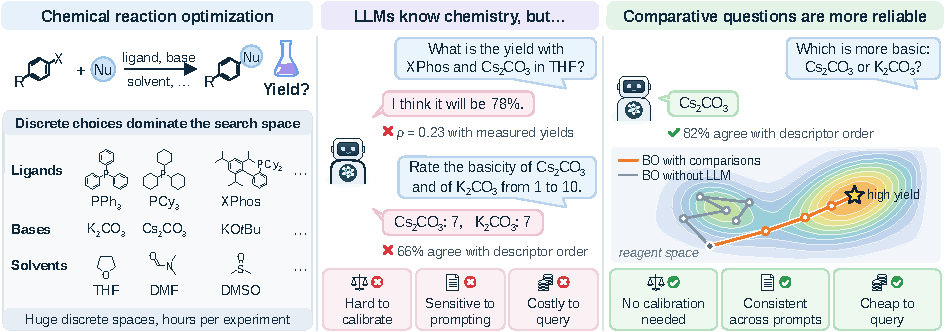
\includegraphics[width=\textwidth]{../shared/figures/fig1_motivation.pdf}
\caption{Ask which, not how much. \textbf{Left:} reaction optimization searches mostly over categorical choices, and each experiment takes hours. \textbf{Middle:} asked for absolute quantities, LLMs predict yields that correlate weakly with measured ones (Spearman $\rho=\PredRho$), and the orderings implied by their 1--10 ratings agree with descriptor orderings for \RateAccPct{} of reagent pairs. \textbf{Right:} asked which of two reagents has more of a named property, the same models agree with the descriptors for \PairAccPct{} of pairs (means over five LLMs on Group A, \S\ref{sec:analysis}). \ours{} builds its BO model on such comparisons; the landscape and trajectories are illustrative.}
\label{fig:teaser}
\end{figure*}
